\section{Experimental Results}\label{sec:results}

\subsection{Motivation}\label{sec:motivation}

The objective of this work is to localize the robot HRP-2 while it is
walking in its environment. We will show in this section that precise
localization on a humanoid robot is both crucial to achieve reliable
trajectory execution and challenging due to humanoid robots specific
features.


Firstly, localization is crucial on a humanoid robot as its position
cannot be controlled directly. Legs motion must be planned, which
makes the assumption that all contacts will be perfect (i.e.\ no
friction) during the movement. This is not the case in practice and
leads to execution errors which cannot be ignored. Moreover, reactive
control algorithms relies on the Linear Inverted Pendulum model which
produces rough trajectories. This increases the differences between
the generated motion and the executed one. Therefore, a reliable
localization algorithm is important to allow reliable trajectory
execution.


Secondly, localization on a humanoid robot is challenging. Mobile
robots odometry can be computed using wheel encoders and give a
reasonable hint on the current robot motion. 2d maps can also be used
to simplify the navigation through indoor environments. This is not
the case on a legged robot on which 3d localization is required and
where no encoder based reliable odometry exists.


Both of these reasons makes localization a cornerstone of reliable
trajectory execution on humanoid robots.


\subsection{Experimental Setup}\label{sec:xp_setup}


\begin{figure}[ht!] %FIXME: this figure is not referenced.
  \begin{center}
    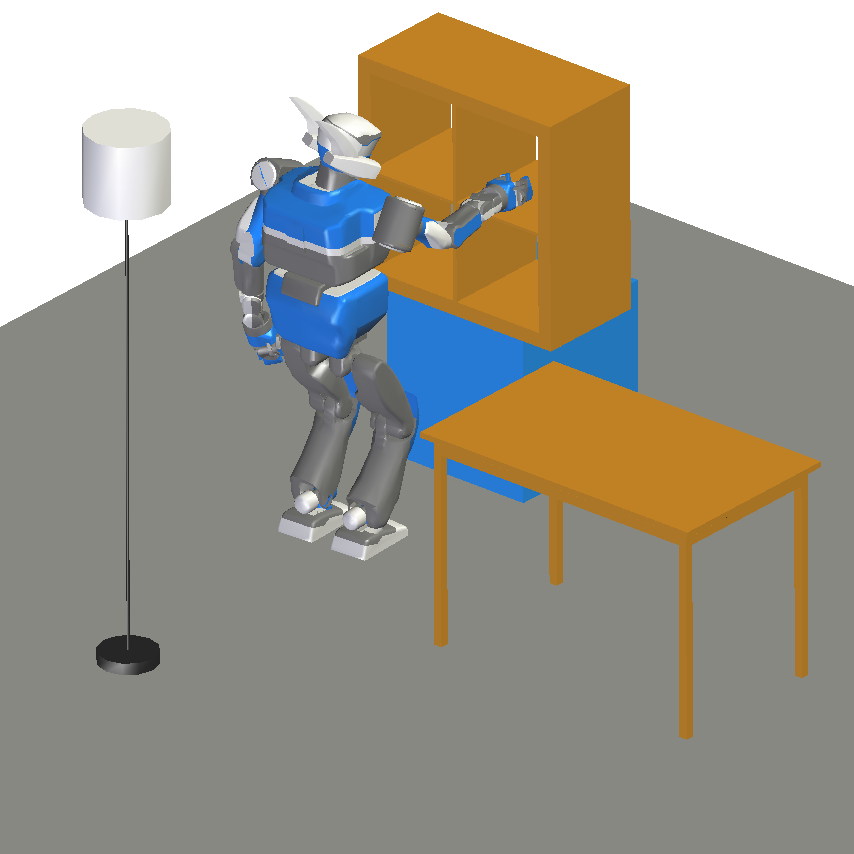
\includegraphics[width=\linewidth]{images/trajectory-8.png}
  \end{center}
  \caption{The HRP-2 robot drops a ball on a shelf while localizing
    itself using visual SLAM. \label{fig:xp_setup_screenshot}}
\end{figure}


The experiment demonstrates that by localizing the robot while
walking, HRP-2 can reach a goal position independently of the
execution errors. In the chosen scenario, the robot must drop a ball
on a shelf after walking 2 meters. A more precise description of the
scenario is Fig.~\ref{fig:xp_setup_dim}. Empirically, we estimated the
HRP-2 mean drift to be around one centimeter per step. Considering
that 32 steps are required to reach the goal without hitting the
obstacles, the usual drift would prevent the task from being
accomplished.

\begin{figure}[ht!]
  \begin{center}
    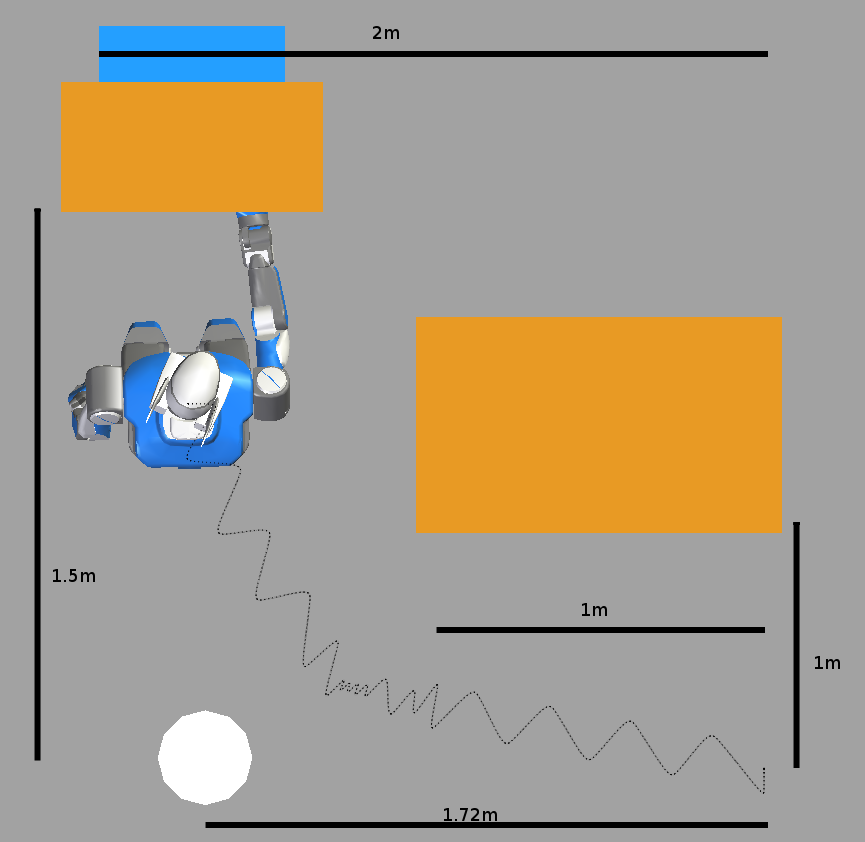
\includegraphics[width=\linewidth]{images/dimensions.png}
  \end{center}
  \caption{Experimental setup description (top view). The dotted line
    displays the robot waist trajectory.\label{fig:xp_setup_dim}}
\end{figure}


The camera trajectory estimated by the visual SLAM algorithm is
validated using motion capture data. Markers have been placed on both
the robot head to provide ground truth.


\subsection{Robotics Framework for Reliable Trajectory Execution}\label{sec:ex_framework}

\begin{figure}[ht!]
  \begin{center}
    FIXME
  \end{center}
  \caption{Complete robotics framework
    overview. \label{fig:framework_overview}}
\end{figure}


The HRP-2 robot embeds two computers. One is dedicated to motor
control and the other one to vision processing. The
Fig.~\ref{fig:framework_overview} illustrates the complete robotics
distributed infrastructure used in this experiment. It relies heavily
on both OpenHRP and ROS to integration the different modules
altogether.


The control is based on a task based controller
\cite{Mansard09icar}. Using a given stack of tasks, this controller
computes the joint velocities $\mathbf{\dot{q}}$ the control which
realizes the tasks. Our stack of tasks ensures that the left ankle,
right ankle, center of mass and upper level posture reference
positions are followed. The reference trajectories are computed
off-line by the planner described in \cite{Dalibard11humanoids}.

This controller reference trajectories can be post-processed to
reshape them on the fly. The controller has been extended to
incorporate a module which can, given an execution error estimation,
cancels them automatically by changing the future robot trajectory.


This estimation of the execution error is computed on the computer
dedicated to vision. By comparing the planned left ankle trajectory
and the estimated one, it is possible to compute an estimation of the
execution error.

The planned left ankle position is computed using both the camera
position and the relative transformation from the camera to the left
ankle. This transformation can be deduced from the robot configuration
and its model using forward kinematics.

To finish, the camera position is given by the visual SLAM algorithm
described in detail in the previous sections. During the experiments,
the acquired image resolution was $320 \times 240$. The localization
module has been running at a mean rate of 16\hertz~during the
experiments. The vision computer running the visual SLAM node is a
Intel\textregistered Core\texttrademark\ 2 CPU T7200~@~2.00GHz with 2Gb.\ of RAM.


\subsection{Comparison to Motion Capture Data}\label{sec:mocap}

The Table.~\ref{tab:mocap_comparison} contains the camera position
estimated by the motion capture system and by the visual SLAM
algorithm. The mean error is FIXME meters and FIXME rads. Drop in the
algorithm precision can occur when the robot enters a part of the map
which is not dense enough or where the environment does not
incorporate enough texture to detect enough interest points.
%FIXME we will see depending on the final data...


The used motion capture system is a Motion Analysis system relying on
six Eagles and four Hawks cameras. It provides an estimation of the
camera position at 200\hertz~with a precision error less than one
centimeter.

%FIXME write conclusion -> summarize results.

\begin{figure}[ht!]
  \begin{center}
    FIXME
  \end{center}
  \caption{Camera position estimated by both the motion capture system
    and the visual SLAM algorithm. \label{tab:mocap_comparison}}
\end{figure}


%%% Local Variables:
%%% ispell-local-dictionary: "american"
%%% LocalWords:  odometry HRP
%%% End:
